% status: 0
% chapter: TBD

\title{Runtime comparasion of application between containorized vs standalone.}

\author{Anubhav Lavania}
\affiliation{%
  \institution{Indiana University}
  \streetaddress{Smith Research Center}
  \city{Bloomington} 
  \state{IN} 
  \postcode{47408}
  \country{USA}}
\email{anubhav.lavania@gmail.com}


% The default list of authors is too long for headers}
\renewcommand{\shortauthors}{G. v. Laszewski}


\begin{abstract}
Docker swarm enables clustering of numerous docker nodes to act as
single virtual machine. It enables clustering and scheduling of
different docker containers. Oracle Virtual box enables running guest
operaing system on top of base operating system and needs dedicated
resources of underlying hardware. In this paper we will comare the
performance of an application when run on Docker swarm and Oracle VM.

\end{abstract}

\keywords{hid-sp18-413, Docker Swarm}


\maketitle


\section{Introduction}

This paper provides a comparasion of running an application in a containerized
environment vs running the same applicatin on a standalone hardware. We will run
an application on a docker swarm cluster~\cite{hid-sp18-413-dockerswarm} of
three raspberry pi's and run the same aplication on a Ubuntu VM using Oracle
Virtual box and compare the performance.

The setup is shown in Figure~\ref{F:setup}.

\begin{figure}[!ht]
  \centering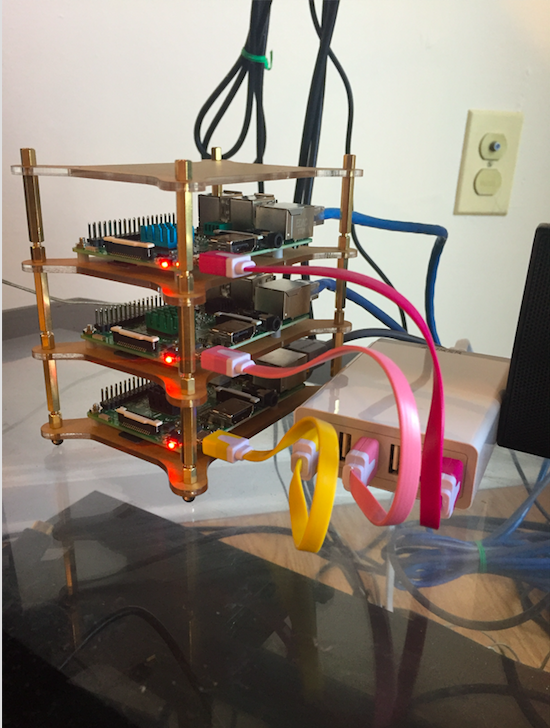
\includegraphics[width=\columnwidth]{images/hid-sp18-413-my3pi.png}
  \caption{my3pihomesetup}\label{F:setup}
\end{figure}

\section{Technologies used}
This section describes the technologies used for building this project
and their brief overview. 

\subsection{OracleVirtual Machine}
~\cite{hid-sp18-413-OracleVM}Oracle Virtual machine is virtualization software by Oracle. Software
is deployed on a guest operating system and it uses dedicated
resources of the host which can be pre-configured during installation
or changed post installation. Guest operating system is deployed using
Oracle Virtual box. It supports most of Unix type OS's like Redhat,
Ubuntu, Debian etc and Macos and windows operating systems. Oracle VM
gives the flexibility to run users applications and programs on
various operating systems without the need to get dedicated hardware
for everyone of them.

\subsection{Docker}

``~\cite{hid-sp18-413-docker} Docker is a tool
designed to make it easier to create, deploy, and run applications by
using containers. Containers allow a developer to package up an
application with all of the parts it needs, such as libraries and
other dependencies, and ship it all out as one package. By doing so,
thanks to the container, the developer can rest assured that the
application will run on any other machine regardless of any customized
settings that machine might have that could differ from the machine
used for writing and testing the code.'' Docker provides the ability to
run application as lightweight and self suffecient code within a
container and therefore provides means for continous integration and
continous development. The difference between docker and Virtual
machine is illustrated in~\ref{f:contvsvm}.

\begin{figure*}[!ht]
	\centering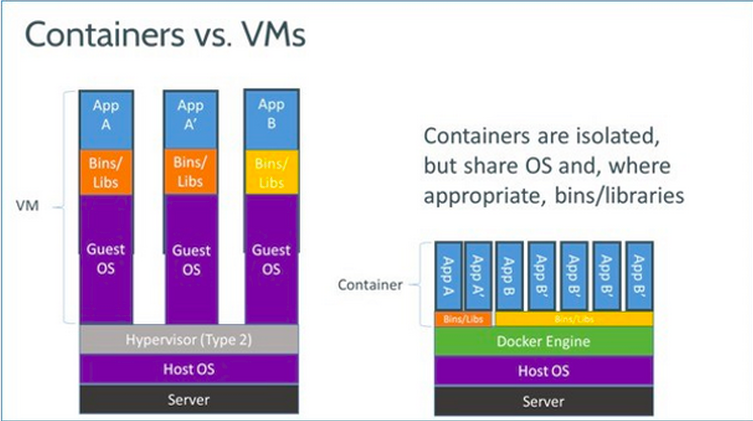
\includegraphics[width=\columnwidth]{images/dockervsvm.png}
	 \caption{Docker VS Virtual Machine}\label{f:contvsvm}
\end{figure*}

\subsection{DockerSwarm}
~\cite{hid-sp18-413-dockerswarm}Docker swarm is the clustering and orchestrization tool from
Docker. It enables running of a dockerized application on multiple
containers and act as if it was running on one. It enables the
application to scale horizontally to hundreds of thousands of
commodity hardware. Docker swarm in addition to scalability provides
inbuilt fault tolerance capabilities. If one or more containers or
servers fail the aplication is seamlessly run on remaining
servers. With Docker swarm application developers and administrators
can add or remove containers on as needed basis. Docker swarm has
manager and worker nodes which are configured at run time. Manager
manages membership and delegation while worker runs swarm services.

\subsection{Dockerhub}
~\cite{hid-sp18-413-dockerhub}Dockerhub is central repository for code repositories and docker
images. You can upload your own image or use officia images. It is
cetralized resource for container images which can be pulled for easy
deployments, distribution and development pipeline. It comes with its
own set of commands like pull, push and search for exploring images.

\section{Hardware used}
\subsection{Macbook Air}
\begin{itemize}
\item Operating: System macos High Sierra
\item Processor: 1.8 GHz Intel Core i5
\item Memory: 8GB 1600 MHz DDR3
\item Graphics: intel HD Graphics 6000 1536 MB
\end{itemize}

\subsection{RaspberryPi}
\begin{itemize}
\item SoC:Broadcom BCM2837 (roughly 50 percent faster than the Pi 2)
\item CPU:1.2 GHZ quad-core ARM Cortex A53 (ARMv8 Instruction Set)
\item GPU:Broadcom VideoCore IV @ 400 MHz
\item Memory:1 GB LPDDR2-900 SDRAM
\item USB ports:4
\item Network:10/100 MBPS Ethernet, 802.11n Wireless LAN, Bluetooth
  4.0
\end{itemize}

\section{Software and packages}
This section gives a brief description of the different softwares and
packages that were used in this projects implementation.

\subsection{python3.6}
``\~cite{hid-sp18-413-python}Python is an interpreted high-level programming language for
general-purpose programming.Python has a design philosophy that
emphasizes code readability, notably using significant whitespace. It
provides constructs that enable clear programming on both small and
large scales. Python features a dynamic type system and automatic
memory management. It supports multiple programming paradigms,
including object-oriented, imperative, functional and procedural, and
has a large and comprehensive standard library.'' Python is easy to use
and is popular for human readability. Just like with every other
programming lanuage each task can be completed in more then one ways
but with python there is a saying of doing it in a PYTHONIC way, which
tells that the approach to solve problems and implement solutions are
sometimes implemented to make it easy to interpret and reduce code complexity.

\subsection{Pandas}
~\cite{hid-sp18-413-pandas}Padas is powerful python library providing high performance, easy to
implement data structures and data analysis tools for Python. Pandas
enables running data analysis effeciently wihhout the need for
switching to other languages. It allows user to focus on
implementation and research part and not get lost in programming aspect.

\subsection{Numpy}
~\cite{}Numpy is matmatical library for Python allowing to work with multi
dimensional arrays, matrices and provides mathmatical functions to
work on different data structures. 

\subsection{Sklearn}
Sklearn is free software library for python providing support for
various classification, regression and clustering algorithms that
include kmeans, vector machines among others. It is written primarily
in python and cython. It is designed to work with other Python data
analysis and math libraries like Numpy and Scipy.


\section{Algorithms}
This section lists the algorithms used for interprating and
claasification of data set used in this project.

\subsection{kmeans}
~\cite{hid-sp18-413-kmeans}kmeans algorithm is used to classify a data set into groups of data
sets that are similar to one another. Groups of data that are similar
are called clusters. Kmeans algorithm stores cluster centers called
centroids(k). A data point belongs to a certaing cluster if it is
closer to its clusters centroid   compared to other clusters.  Kmeans
works by assigning and reassigning centroids to cluster untill no more
reassignment can be done. This is achived by assigning assigning data
points to clusters based on the current centroids and then chosing
centroids based on the current assignment of data points to
clusters. Goal of algorithm is to Initialize k means with random
values. 1 Pick K random points as cluster centers called centroids.2 Assign each xi
 to nearest cluster by calculating its distance to each centroid.3  Find new cluster center by taking the average of the assigned points.4 Repeat Step 2 and 3 until none of the cluster assignments change.
\paragraph{Algorithm}
We are provided with a data set ${x^{(1)}, .. , x^{(n)}}$ and want
to group this data into cluster. We need to predict k centroids and a
label $c^{(i)}$ for each data point. The kmeans algorithm is:

\begin{figure*}[!ht]
	\centering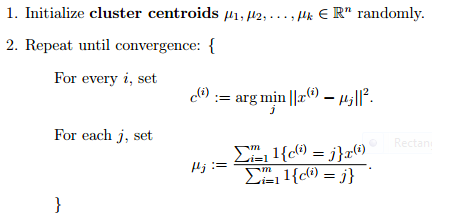
\includegraphics[width=\columnwidth]{images/kmeans.png}
	 \caption{Kmeans Algorithm}\label{f:kmeans}
\end{figure*}
where $\b{c}_i$ is the set of points that belong to cluster i. The
K-means clustering uses the square of the Euclidean distance
$d(\b{x},\mu_i) = \left\Vert \b{x}-\mu_i \right\Vert_2^2$ 

\begin{figure*}[!ht]
	\centering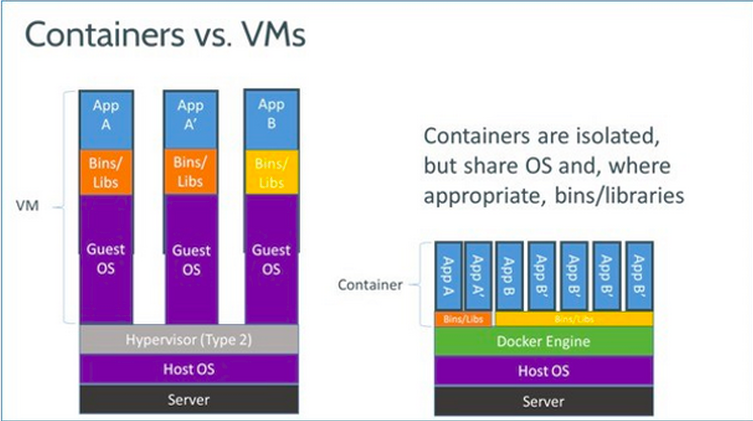
\includegraphics[width=\columnwidth]{images/dockervsvm.png}
	 \caption{ClusterFormation}\label{f:clustering}
\end{figure*}

\section{RaspberryPi Setup}
First we need to get Raspbian onto an SD card. This means downloading
the raspbian operating system and putting it on a sd card which will be
installed on raspberry pi. Sd crad card reader is inbuilt in most
laptops or desktops. Download etcher for your operating system and
burn the raspbian os image on the sd card using etchers
interface. Once it is complete install sd card into the pi. Continue
doing the same for all sd cards. Install sd cards onto raspberry
pis. Connect ethernet cables to all respberry pis making sure that
they do not touch each other and connect the cables to a network
switch. Better to use a stackable case to prevent pi's touching each other. 
Attach usb power cables to all pi's and you should see a red led
indicating that pi's are powered up. Run nmap utility to scan all the
ip addresses on network and identify new ones and ssh to pi using the
ip address. Best practise to do first thing is to change the default
password. Also update etc/hosts file with jostnames and ipaddres of
newly installed pi's. Use ssh-keygen to generate ssh keys and copy
them over to other pi's.
\subsection{Implementation}
Import kmeans, numpy and pandas packages. Load the sample data using
pandas library. Zp the values in two numpy arrays. Define the number
of clusters you want the data to be divided into. Predict the clusters
and get the centroids. Following are the runtimes of running my
program when generating x number of clusters for same data set.\\
x = 4. Total runtime is  0.06981004799308721\\
x=10. Total runtime is  0.22681947400269564\\
x=50. Total runtime is  0.5675595289940247\\
x=100. Total runtime is  0.9938862379931379\\
x=200. Total runtime is  1.7820694190013455\\
x=500. Total runtime is  4.269817592008621\\
x=1000. Total runtime is  8.043557413999224\\
x=2000. Total runtime is  17.261475505001727\\
x=3000. Total runtime is  25.911107341991737\\
If the number of clusters exceeds data rows, program exits with an
error. \\
Kmeans algorithm is pretty useful in seperating the data into similar
data clusters. It uses calculating eucladian distance formula and works well for well
structured data. But it has its own shortcomings. The results produced
depend on initial values for means which derive the final
output. It is highly difficult to determine how many clusters are
optimal for a given data set.

\section{Conclusion}
Here we observe that program runtime is proportional to number of
clusters when running the program on a VM. Due to issues with setting
up docker swarm cluster on raspberry pi there is no data available for
a comparasion as of now. Author will conitnue this work to implement
the solution of docker swarm cluster and do the comparasions. 


\begin{acks}

  The authors would like to thank Dr.~Gregor~von~Laszewski for his
  support and suggestions to write this paper.

\end{acks}

\bibliographystyle{ACM-Reference-Format}
\bibliography{report} 

